\section{Quadcopter flight tests}

Once the performance and safety of the control algorithms has been validated in the simulated environment, it is possible to begin flight tests and take to the air with a physical drone.
In this final section of the validation process, all the previous parts are put together in order to test how the developed software will perform in a real quadcopter during flight.
To do this, first it will be necessary to be build the base vehicle from its development kit and then integrate all the additional pieces needed for this project, like the companion computer and the camera.
Then, after making sure that the vehicle can fly with all the payload through remote control, both of the developed solutions will be tested:
first the hand-control solutions to verify that the autopilot can receive flight commands from an offboard computer and second the follow solution to verify that the companion computer can function as well during flight with its dedicated power supply as it did when it was stationary.

The exact steps that will be executed one after the other to ensure that safety is maintained during the whole process are as follows:

\begin{enumerate}
    \item Build the quadcopter with its basic components.
    \item Add custom payload.
    \item Fly with remote control and factory autopilot only, monitoring through QGRoundControl.
    \item Fly with custom software from offboard computer with test tool \verb|test-camera| \ref{subsec:test-tools}.
    \item Fly with test tool \verb|test-camera| from onboard computer.
    \item Fly with custom hand-gesture control solution from offboard computer.
    \item Fly with custom follow solution from onboard computer.
\end{enumerate}

\subsection{Build process}
\label{sec:test-7-builddrone}

% Setup:    build drone, configuration, calibration
% Test:     - RC, GPS, 
%           - Arm, takeoff commands
%           - Camera holder
% Results:  wiring, drone pictures, QGroundControl calibration screens
%           holder 3d, drone close-up, camera feed


As has been mentioned before, the vehicle used in this project is the Holybro X500, designed specifically to work with PX4.
The detailed instructions to build the vehicle from its Development Kit can be found in the PX4 documentation \footnote{\url{https://docs.px4.io/main/en/frames_multicopter/holybro_x500_pixhawk4.html}}.
Figure \ref{fig:x500-dev-kit} shows all the parts that make up the complete vehicle.

\begin{figure}
  \centering
  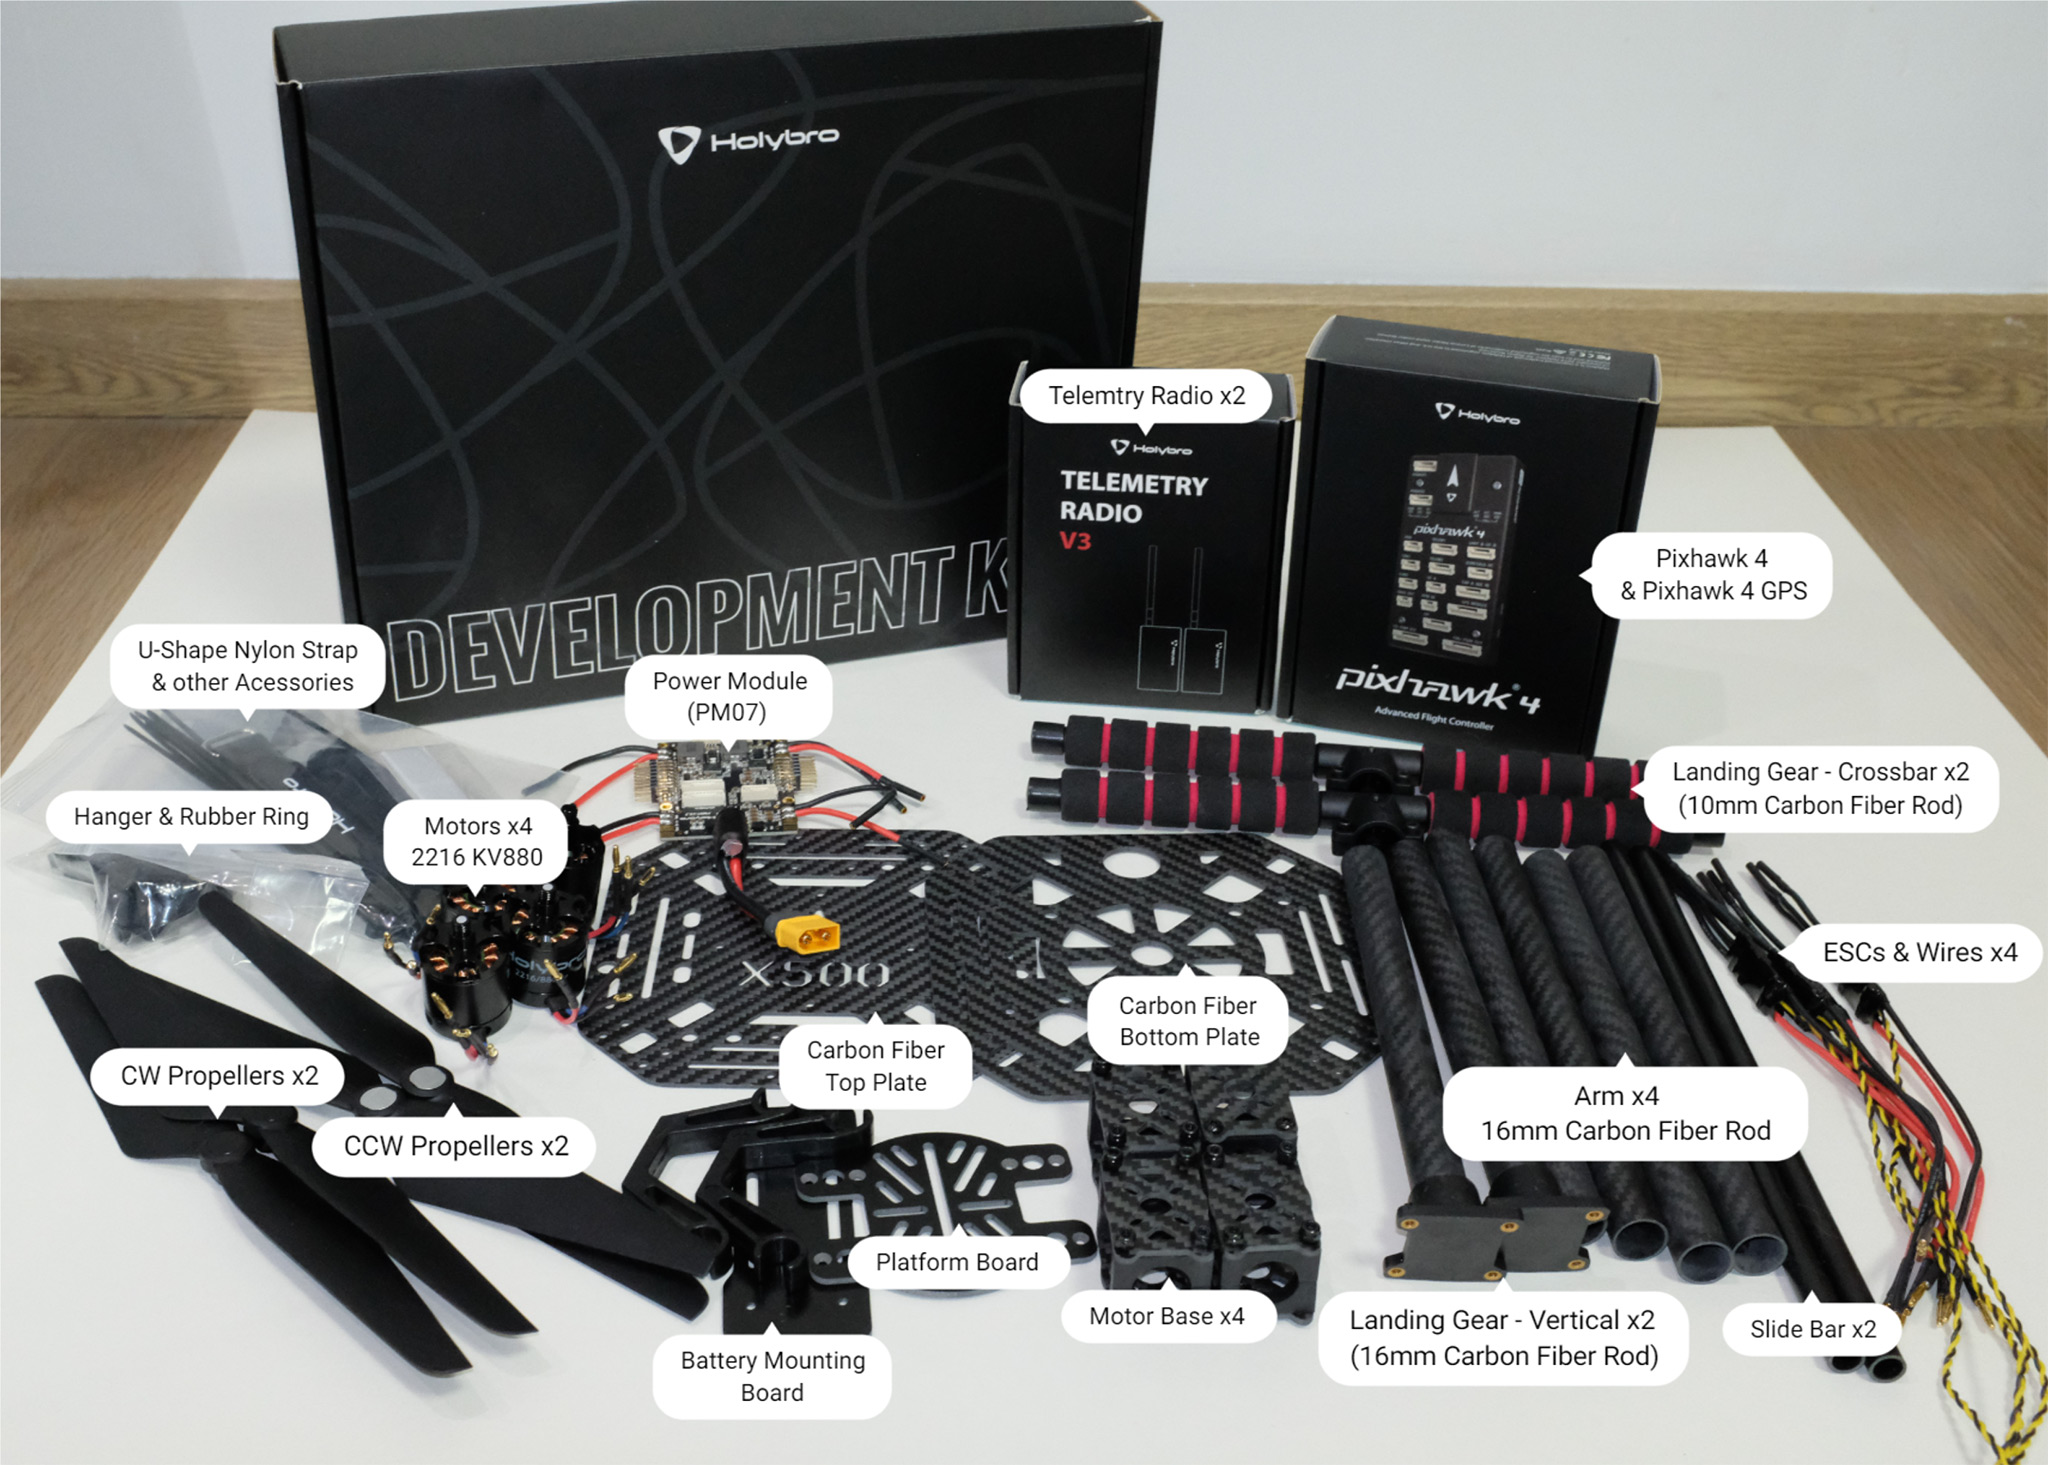
\includegraphics[width=.6\textwidth, keepaspectratio]{img/x500-dev-kit.jpg}
  \caption{Development kit for the Holybro X500}\label{fig:x500-dev-kit}
  \todo{Cite}
\end{figure}


After all the standard parts are put together, the custom additions can be attached as well using the remaining space in the frame.
The Raspberry Pi companion computer will sit just behind the autopilot to counterbalance the more weighted front of the vehicle where the GPS-antenna is located.
This location also allows an easy connection between the autopilot and Raspberry's I/O pins with short cables, so as not to clutter the frame with wires excessively.

While in flight the Raspberry Pi will be powered through a dedicated external battery that outputs power through a 2-ampere USB port.
This port will be connected with the Raspberry Pi's original power cable to its USB-C power supply socket.
As detailed in \ref{sec:test-5-rpi}, this current is enough to power the connected camera and run the developed software with an acceptable performance.
This battery will be located underneath the autopilot, centered in the frame of the vehicle so its weight destabilizes it as little as possible, as can be seen in figure \ref{fig:full-build}.

The camera also needs to be attached to the frame of the vehicle in a secure way.
For this purpose, a support has been designed and 3D-printed from PLA plastic.
The holder attaches to the slide bars underneath the main frame of the vehicle so that the camera and its substantial weight is situated as close to the center of mass as possible, behind the GPS platform.
The battery powering the engines and the autopilot, which is located on the underside of the carbon frame, is also moved slightly backwards from its centered position to make space for the camera and compensate its weight in the front.
Figure \ref{fig:camera-holder-closeup} shows how the underside of the vehicle looks with the camera attached.
The 3D model of the custom support can be seen in figure \ref{fig:camera-holder-3d} and the print-ready file can be found in the project repository in GitHub. \todo{Link 3D model in repo}

\begin{figure}
  \centering
  
\includegraphics[width=0.8\textwidth, keepaspectratio]{img/placeholder.png}
  \caption{Full build annotated with arrows}\label{fig:full-build}
\end{figure}

\begin{figure}
  \centering
  
\includegraphics[width=0.8\textwidth, keepaspectratio]{img/placeholder.png}
  \caption{}\label{fig:camera-holder-closeup}
\end{figure}

\begin{figure}
  \centering
  
\includegraphics[width=0.8\textwidth, keepaspectratio]{img/placeholder.png}
  \caption{}\label{fig:camera-holder-3d}
\end{figure}


After the vehicle has been built, there are additional installation and calibration steps that must be carried out before it can fly, also contained in the guide mentioned above.
The QGroundControl \ref{subsec:qgc} ground station application contains a configuration screen with all the calibration tools needed for the vehicle setup, as shown in figure \ref{fig:qgc-config}.
The vehicle can be configured either by connecting the flight controller directly to the computer via the micro-USB port on its side or through a wireless connection by plugging the companion telemetry radio to the computer running QGroundControl.
Before any flight can be carried out, any simulation modes previously activated for testing must be deactivated from the Safety section of the vehicle configuration.


\begin{figure}
  \centering
  
\includegraphics[width=\textwidth, keepaspectratio]{img/placeholder.png}
  \caption{Screenshot from the QGroundControl calibration and setup tools used to configure the vehicle}\label{fig:qgc-config}
\end{figure}


\subsection{Basic tests}
\label{sec:test-8-flight}

% Setup:    flight plan
% Test:     - assisted takeoff, fly with RC
%           - tools/test_camera + record video
% Results:  video of flying, adjust pid set-point

\subsubsection{Baseline flight with factory software}

Once the vehicle is fully configured, the RC controller and QGroundControl can be used to test assisted take off and landing.
At this point, the drone should be able to maintain stable flight while using autopilot-assisted flight modes like Position Mode, where the roll and pitch sticks control the acceleration over ground of the vehicle in the forward/backward and left/right directions relative to the heading the vehicle is facing, and throttle controls speed of ascent and descent. 
With the sticks centered the vehicle will actively remain locked to a position in 3D space, compensating for wind and other forces.
This is the safest manual mode to test that the standard autopilot is working as expected.

Through QGroundControl it is possible to map the different switches in the RC controller to different autopilot commands.
For this test, one of the switches with two positions will be mapped to arm/disarm, which controls whether the engines of the quadcopter can start or not, and one of the switches with three positions will be mapped to the landing/takeoff/position flight modes respectively, so the main autopilot modes can be tested by moving the switch between the available positions during flight.
This configuration exhausts all the channels available in the RC controller employed.
Other flight modes can be set by using the QGroundControl interface directly.

To carry out the flight, first the main battery is connected to the socket in the power module.
This starts up the autopilot, the GPS antenna, the telemetry radio and the RC receiver.
Afterwards, QGroundControl can be started in a computer that has been connected to the second telemetry radio via USB.
If everything has worked correctly, the ground station application will automatically connect to the vehicle and situate its position in a satellite map.
Turning on the RC controller will likewise make it connect to the vehicle, as long as it has been paired correctly as indicated in the guide linked in the first step of the build process.
Once all the wireless connections have been established the drone can take off by first switching to the armed state and then switching to the takeoff flight mode.
While the drone is in the air, switching to the position flight mode will allow direct control through the joysticks in the controller.
Figure \ref{fig:flight-test-basic} shows an image from a flight carried out following this steps.
The full video of the test can be seen in link \todo{Make video and link}.

\begin{figure}
  \centering
  
\includegraphics[width=.6\textwidth, keepaspectratio]{img/placeholder.png}
  \caption{Picture from flight tests}\label{fig:flight-test-basic}
\end{figure}

\subsubsection{Offboard computer flight with test tool}

The second test flight will aim to make certain that the custom software can send takeoff and landing commands through a wireless MAVlink channel from the offboard computer (by using the telemetry radio through the developed test tool).
For this flight, the QGroundControl application cannot be connected to the vehicle since the telemetry radio channel will be blocked by the custom tool.
The RC controller will be therefore be used as a backup in case anything goes wrong with the software.
At any moment the controller can switch flight mode and override the input generated from the dronecontrol application, recovering manual control.
Now, once the main battery is connected again to the power module, the test tool is run with the command \verb|dronecontrol tools test-camera -r COM<X>:57600| on a Windows PC or with \verb|dronecontrol tools test-camera -r /dev/ttyUSB0:57600| on a Linux computer.

After a successful connection to the vehicle, the T and L keys in the computer keyboard can be used for takeoff and landing, respectively, and the O key can be used to set the autopilot in offboard flight mode to make it able to receive velocity commands.
Afterwards, the WASD keys can be used to control the forward and sideways velocity of the vehicle and the QE keys to control its yaw velocity.
Figure \ref{fig:flight-test-cam-offboard} displays the output on the terminal window of the computer, where the connection process and the sent velocity commands are shown, and the output on the camera from the offboard computer.

\begin{figure}
  \centering
  
\includegraphics[width=.45\textwidth, keepaspectratio]{img/placeholder.png}
  
\includegraphics[width=.45\textwidth, keepaspectratio]{img/placeholder.png}
  \caption{a) Terminal output from the test-camera tool running on an offboard computer and b) Output from the camera of the offboard computer towards the vehicle in flight}\label{fig:flight-test-cam-offboard}
\end{figure}

\subsubsection{Onboard computer flight with test tool}

The third and last test flight in this section will ensure that the custom software can send takeoff and landing commands through a cabled MAVlink channel from the onboard computer,
as well as making sure that the onboard camera can obtain a good image of the field of view of the vehicle during flight.
For that, the same tool will be used as in the last test, 
but in this instance it will be run on the Raspberry Pi and the connection will be established through the wired serial link between this onboard computer and the Pixhawk autopilot board.
Since the camera connected to the computer sending commands is now looking down on the pilot, it is also possible to activate pose detection on the test images received from this onboard camera.
To start the flight test, the main battery and the secondary battery need to be attached, respectively, to the power module and to the Raspberry Pi.
After the onboard computer has started up, the easiest way to take control of it is with a remote desktop connection through WiFi, as explained in section \ref{sec:devenv}.
By this connection, a terminal window can be opened on the desktop and the following command run:
\verb|dronecontrol tools test-camera -r /dev/serial0:921600 -p|
As opposed to the flight using the telemetry radio, in this test the serial connection runs at a baudrate of 921600, which matches the configured baudrate on the \verb|TELEM2| port of the Pixhawk board.
The "-p" option is used to enable pose detection in the output images.
The terminal and camera output can be seen in figure \ref{fig:flight-test-cam-onboard} and a video recording the remote desktop during the flight can be seen in link \todo{Link video of screen during onboard test-camera flight}.


\begin{figure}
  \centering
  
\includegraphics[width=.6\textwidth, keepaspectratio]{img/placeholder.png}
  \caption{Pose detection algorithm running on images taken during flight}\label{fig:flight-test-cam-onboard}
\end{figure}


\todo[inline]{lint all commands on this section properly, consistent \\verb|| on test-camera }

\subsection{Hand gesture control}
\label{sec:test-9-hand}

% Setup:    ...
% Test:     - Hand solution on windows through telemetry radio
%           - Free movement with offboard api
% Results:  video of flying, output from program

During basic flight tests, all the connections and individual parts of the software were validated in real flight.
Now it is time to integrate the piloting system with the image recognition results to test the vision-based control solutions developed.
The first solution to be used in flight will be the hand-gesture guidance system, as it is made to run on an offboard computer with more available processing resources and no dependence on battery-supplied power to work.
The setup will be identical to the second test flight with the telemetry radio as the serial link and the onboard companion computer turned off
Once the autopilot board is powered up, the control solution can be started with the following command:
\verb|dronecontrol hand -s <device>:57600|
where <device> is the COM port or TTY device the telemetry radio is attached to, depending on the platform.


After the pilot connects, the image from the webcam of the computer will appear on the screen with an outline over any detected hand.
To start controlling the vehicle, an open palm should be shown to the camera.
Then, a closed fist will make the drone take off and pointing up with the index finger will start offboard flight mode.
Afterwards, moving the index finger right or left will make the vehicle mirror the movement, 
and moving the thumb right or left will make the vehicle move forwards and backwards, respectively \todo{Check direction of thumb movement}.
At any point during the test, an open hand will make the vehicle land at the current place and losing sight of the controlling hand will make the vehicle return to the starting position before landing as well.
\todo[inline]{Make return home altitude less before flying}

\todo[inline]{Video should show side-by-side computer screen with terminal and image output and video from vehicle flying, synced}

\begin{figure}
  \centering
  
\includegraphics[width=.6\textwidth, keepaspectratio]{img/placeholder.png}
  \caption{Image taken during flight controlled by the hand-gesture solution. Vehicle is taking off}\label{fig:flight-test-cam-onboard}
\end{figure}

\begin{figure}
  \centering
  
\includegraphics[width=.6\textwidth, keepaspectratio]{img/placeholder.png}
  \caption{Image taken during flight controlled by the hand-gesture solution. Vehicle is moving to the right.}\label{fig:flight-test-cam-onboard}
\end{figure}

\begin{figure}
  \centering
  
\includegraphics[width=.6\textwidth, keepaspectratio]{img/placeholder.png}
  \caption{Image taken during flight controlled by the hand-gesture solution. Vehicle is moving forward}\label{fig:flight-test-cam-onboard}
\end{figure}

\subsection{Target detecting, tracking and following}
\label{sec:test-10-follow}

% Setup:    ...
% Test:     - Follow solution on RPi
%           - Controller response to real input
% Results:  video of flying, output from program
